% !TEX root = CSUR/main.tex

\section{Introduction}

Symbolic execution is a powerful program analysis technique introduced in the mid 70's in the context of software testing (see, e.g.,~{\cite{K-CACM76} and~\cite{H-TSE77}})\mynote{IF: are references appropriate? Should we give more credits? It seems several groups introduced independently this technique}. The basic idea is to allow the program to take on ``symbolic'' -- instead of concrete -- input values. Variables and control flow paths are associated with expressions and constraints in terms of those symbols during a symbolic execution of the program, and constraints are eventually solved via SMT (satisfiability modulo theories) solvers.

In this article we survey the main aspects of symbolic execution and discuss its extensive usage in computer security applications\mynote{IF: want focus on security?}, where software vulnerabilities can be found by symbolically executing programs at the level of either source or binary code.
We start with a simple example that will introduce many of the fundamental issues discussed in remainder of the paper.

\begin{figure}[t]
\centering

\includegraphics[width=0.35\columnwidth]{images/concrete-abstract.eps} 
\caption{Concrete and abstract excution machine models.}
\label{fig:concrete-symbolic}
\end{figure}

\subsection{Warm-up example}
\label{symbolic-execution-example}

Consider the simple C function shown in Figure~\ref{fig:example-1}, whose most critical operation is the division at line 10. Each of the input values {\tt a}, {\tt b}, and {\tt c} can be assigned with $2^{32}$ distinct integer values, though only values leading to $x + y + z - 3 = 0$ make the code crash. While techniques such as random testing could generate bottomless input tests for this function, it is unlikely that exactly the crash-inducing inputs would be randomly picked up\mynote{Fuzzing?}. 
Symbolic execution overcomes these limitations by evaluating a piece of code using {\em symbols}, instead of concrete values, for its inputs. This makes it possible to reason on {\em classes of input values}, instead of single input instances. 

\begin{figure}[t]
\begin{lstlisting}[basicstyle=\ttfamily\small]
              1.  int foobar(int a, int b, int c) {
              2.    int x = 0, y = 0, z = 0;
              3.    if (a != 0)
              4.      x = -2;
              5.    if (b < 5) {
              6.      z = 2;
              7.      if (a == 0 && c != 0)
              8.        y = 1;
              9.    }
             10.    return a / (x + y + z - 3);
             11.  }
\end{lstlisting}
\caption{Simple C function used in the warm-up example.}
\label{fig:example-1}
\end{figure}

In more details, every global or local variable is associated with a symbol $\alpha_i$.  At any point of the execution, the symbolic engine maintains:

\begin{itemize}
  \item  an execution state $(stmt,~pc)$ where:
\begin{itemize}
  \item $stmt$ is the statement to evaluate. For the time being we assume that $stmt$ can be an assignment, a conditional branch or a jump (a discussion of more complex constructs for iteration and function calls will be provided in Section~\ref{example-discussion});
  \item $pc$ is a collection of path\mynote{IF: my feeling is that pc does not denote a set. Better notation? Isn't pc a logical formula?} constraints, i.e., a set of assumptions made over the symbols $\alpha_i$ in order to reach $stmt$. Initially $pc$ is empty, and is thus trivially satisfied.
\end{itemize}
\item a {\em memory mapping} $M$ for storing constraints over different symbols. This is required since in general every memory location can be associated with a symbol\mynote{Rephrase}.
\end{itemize}

\noindent Depending on $stmt$, the symbolic engine modifies the state as follows:
\begin{itemize}
  \item $stmt$ is a constant assignment $\alpha_i = c$: when a constant value $c$ is assigned to a variable associated to the symbol $\alpha_i$, $pc$ is extended by adding a constraint on $\alpha_i$:\mynote{Redundant? IF: I would remove the constant assignment}
    \[ pc \gets pc \wedge \alpha_i = c\]

  \item $stmt$ is an assignment $\alpha_i = e$: when an expression $e$ is assigned to a symbol $\alpha_i$, $pc$ is extended by adding a constraint on $\alpha_i$:
    \[ pc \gets pc \wedge \alpha_i = e\]
  where $e$ can be any expression, involving unary or binary operators, over symbols and constants.

  \item $stmt $ is a conditional branch ${\tt if}~e~{\tt then}~s_{true}~{\tt else}~s_{false}$: $pc$ is evaluated. Two scenarios are possible:
    \begin{itemize}
      \item (non-forking) $e$ is evaluated as always true or false under the assumptions in $pc$: the proper branch is taken, and symbolic execution advances to $s_{true}$ or $s_{false}$ accordingly;
      \item (forking) $e$ cannot be evaluated without instantiating values for one or more symbols in it: the symbolic execution process is forked, creating two execution states:
        \[ (s_{true}, pc_{true}) \text{ where } pc_{true} = pc \wedge e \]
        \[ (s_{false}, pc_{false}) \text{ where } pc_{false} = pc \wedge \neg e \]
    \end{itemize}
    Symbolic execution proceeds on both states in parallel.

  \item $stmt $ is a jump {\tt goto} $s$: execution state is updated to advance symbolic execution to $s$. 
\end{itemize}

%\subsection{Example}
%\label{symbolic-execution-example}

\begin{figure}[t]
  \centering
  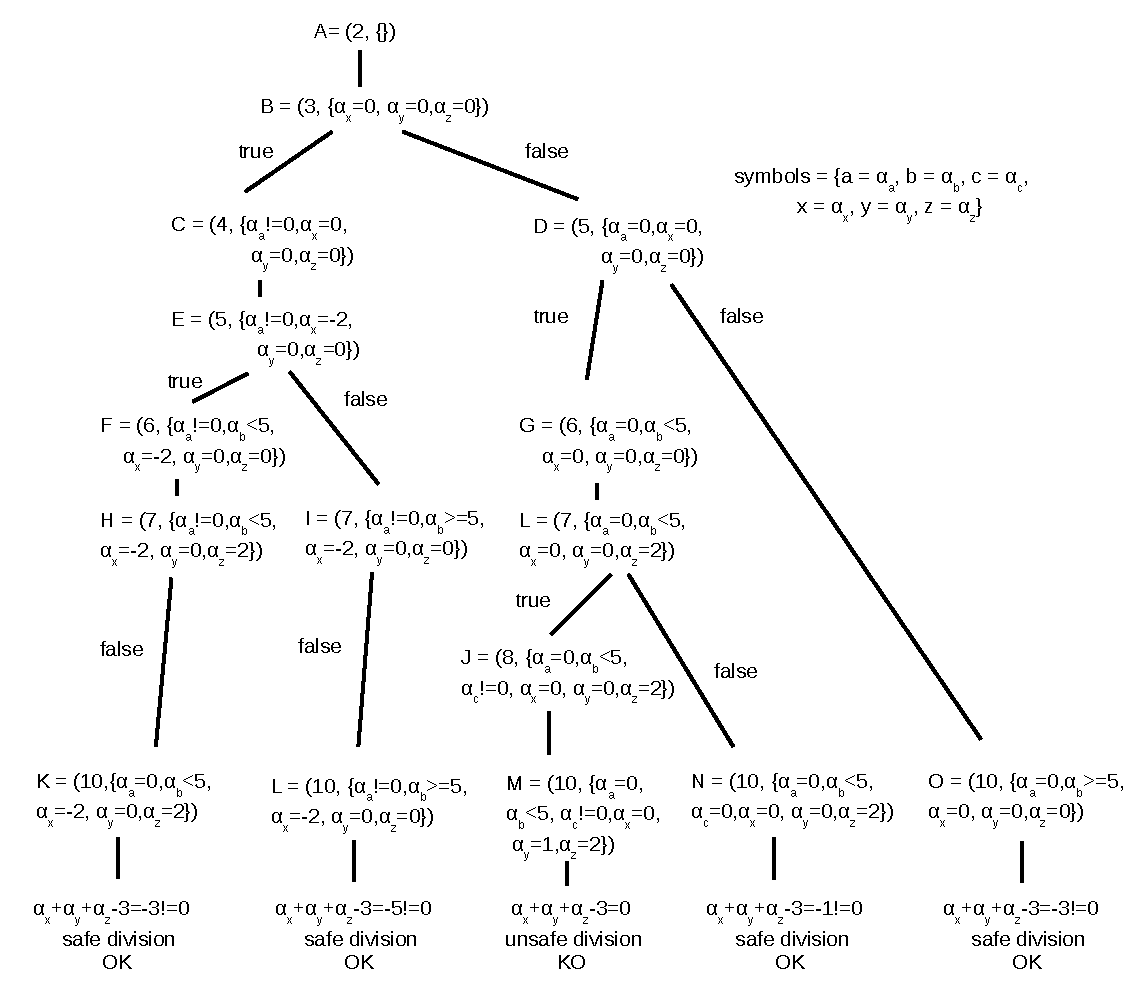
\includegraphics[width=1.0\columnwidth]{images/example} 
  \caption{Symbolic execution tree of the function {\tt foobar}. Each execution state is labeled with an alphabet letter. Side effects on execution states are highlighted in gray. Leaves are evaluated against division by zero error. For the sake of presentation the conjunction of constraints is shown as a list of constraints. }
  \label{fig:example-symbolic-execution}
\end{figure}

A symbolic execution of the function {\tt foobar} is shown in Figure~\ref{fig:example-symbolic-execution}. Initially, a new symbol is introduced for each input argument and for each local variable. For the sake of the presentation, we associate a symbol $\alpha_{var}$ with each variable $var$. 
Moreover, we assume that the set of local\mynote{locals only right? I added "at each point"} variables in use at each point by the function is known. In general, obtaining this information may be non trivial, and symbols are typically introduced when statements defining the variables are reached.
%Moreover, we have assumed to know the set of local variables used by the function. In general, obtaining this information may be non trivial and thus it it common to introduce symbols related to local variables only when the statements defining the variables are evaluated.
We also maintain a mapping table to track the mapping between variables and symbols. 

The first statement of the function is located at line 2. For this reason, the initial execution state $A$ is given by $(2, \{\})$ where the path constraint set is empty as no assumption is made on any symbol. After executing line 2,  $pc$ is updated by adding constraints on the value of $\alpha_x$, $\alpha_y$, and $\alpha_z$ (execution state $B$). Line 3 contains a conditional branch: since the condition cannot be uniquely determined based on the current set of assumptions, the execution is forked. Depending on the branch taken, a different statement is evaluated next and different assumptions are made on the symbol (execution states $C$ and $D$). On the other hand, when a condition can be uniquely determined (e.g., as in execution state $H$), it is sufficient to follow only the relevant branch (e.g., going to state $L$ from $H$), thus pruning unrealistic execution states. 

After expanding every execution state until the statement on line 10 is reached, we can check which input values for parameters {\tt a}, {\tt b}, and {\tt c} can make the function {\tt foobar} crash as a consequence of a division-by-zero operation. Analyzing execution states $\{L, M, N, O, P\}$, we can conclude that only $N$ can lead to an unsafe operation. The path constraint set for $N$ thus defines\mynote{implicitly defines?} the set of inputs that are unsafe for {\tt foobar}. Indeed, any input values for $\alpha_a$, $\alpha_b$, and $\alpha_c$ such that:
 \[ \alpha_a = 0 \wedge \alpha_b < 5 \wedge \alpha_c \neq 0 \]
will make the function crash. An instance of unsafe input parameters for {\tt foobar} can determined exploiting a constraint solver (i.e., an oracle able to resolve constraints). For instance, given the execution state $N$, a solver may come up with the values $a = 0$, $b = 1$, and $c = 0$. Notice\mynote{Say earlier?} that a constraint solver is also needed when evaluating the satisfiability of branch conditions.

\subsection{Discussion}
\label{example-discussion}

The example described in Section~\ref{symbolic-execution-example} shows the effectiveness of symbolic execution in identifying {\em all} the possible unsafe input values that can trigger a crash due to an unsafe division performed at line 10. This is achieved through an exhaustive exploration of all the possible execution states. For this reason, symbolic execution is a sound and complete methodology from a theoretical perspective. Soundness guarantees that input values deemed as unsafe are actually unsafe, and completeness implies that all possible unsafe inputs will be found. However, challenges that symbolic execution has to face when processing real-world code can be significantly more complex compared to those from our toy example of Figure~\ref{fig:example-1}. Several observations and questions naturally arise:

\begin{enumerate}

  \item (objects) {\em How does symbolic execution handle arrays or other more complex objects?} \\
  In general, any arbitrary complex object can be seen as an array of bytes, where each byte is associated with a distinct symbol. In principle, even a C {\tt int} variable can be seen as an array of four bytes.\mynote{Cosa intendiamo qui?} However, it is convenient to exploit structural properties of the data when possible (e.g., by statically analyzing the source code). For instance, for object-oriented languages the search performed by symbolic execution can be refined taking advantage of relational bounds on class fields.

  \item (loops) {\em How does symbolic execution handle loops?} \\
  In the execution model presented in Section~\ref{simple-execution-model} a loop can be encoded as a combination of conditional branches and $goto$ statements. This transformation is frequent when lowering a high-level language like C to an intermediate representation or native code. When the number of loop iterations cannot be determined in advance (e.g., it depends on an input parameter), for a symbolic execution engine choosing how many iterations should be analyzed becomes critical. The naive approach of unrolling iterations for every valid index bound leads to a very large number of states. It is possible to limit the number of iterations to $k$, thus trading speed for completeness, or when loop invariants can be inferred through static analysis they can be used to merge equivalent states (\mynote{Recuperare citazione}e.g., when differences are not observable outside the loop body).

  \item (subroutines) {\em How does symbolic execution handle subroutines?} \\
  Our execution model does not handle invocation of subroutines (i.e., a $call$ statement). \mynote{Extend this paragraph} A way to extend it to support subroutines is to provide the execution state with a simple execution stack.

  \item (recursion) {\em How does symbolic execution handle recursion?} \\
  Consider, as an example, the code:
    \begin{lstlisting}[basicstyle=\ttfamily\small]
    1.  int bar(int n) {
    2.    if (n >= 0) 
    3.      return 0;
    4.    return 1 + sum(n - 1);
    5.  }
    \end{lstlisting}
  Assuming that an execution stack has been added to the state, we observe that this code can easily lead to a very large number of execution states (i.e., a new state is subsequently created every time the branch on line 2 is not taken). As an {\tt int} variable can have up to  $2^{31} - 1$ positive values, symbolic execution has to create as many execution states to cover all the possible execution paths.
 %Indeed, the number of executions states is related to the number of times that the conditional branch on line 2 is not taken. 
 
  \item (environment) {\em How does symbolic execution handle interaction with the environment}? \\
  Real-world applications interacts constantly with the environment (e.g., filesystem, network) through libraries or system calls. A crucial aspect of these interactions is that they may cause side-effects
% on the environments 
(e.g., creation of a file)
%or initialization of a memory area
that must be taken into account, as they may later affect the 
%actual
execution of the code. Evaluating any possible outcome of an interaction is typically not feasible due to the large number of possibly generated execution states, only a small number of which can actually happen in a non-symbolic scenario. Hence, it is common to create models for popular library and system routines that help the symbolic execution engine to consider only significant outcomes.

  \item (state space explosion, path selection) {\em How does symbolic execution deal with path explosion}? \\
  A relatively simple code such as function {\tt foobar}, which is composed by less 12 lines of code, has generated 16 execution states, where $5$ out of $16$ are independent\mynote{Independent?} and must be checked to determine possible unsafe input values. Although this could seem a reasonable number of states, language constructs such as loops may contribute to increase the number of states exponentially. For this reason, it is unlikely that a symbolic execution engine is able to exhaustively explore all the possible execution states within a reasonable amount of time. In practice, heuristics are used to guide exploration and prioritize certain states first (e.g., to maximize code coverage), hoping this would lead to interesting discoveries. Also, a symbolic execution engine should implement efficient mechanism for evaluating multiple execution states in parallel without running out of resources.
  %In practice, several heuristics must be exploited to prioritize evaluation of some states, hoping to still be able to spot interesting things. Moreover, the symbolic execution engine should include efficient mechanism for efficiently evaluating in parallel different execution states without running out of computational resources.

  \item (constraint solver) {\em What can a constraint solver do in practice?}
  %{\em What is a constraint solver in practice}? \\
 Constraint solvers suffer from a number of limitations. Typically, they can handle complex constraints in a reasonable amount of time only if they are made of linear expressions over their constituents. Symbolic execution engines typically implement a number of optimizations to make queries as much {\em solver-friendly} as possible, for instance by splitting queries in independent components to process separately or by performing algebraic simplifications.

  \item (binary code) {\em What are the disadvantages of symbolically executing binary code}? \\
  The example presented in Section~\ref{symbolic-execution-example} is written in C. This does not imply that symbolic execution cannot be performed directly on binary code, which in several scenarios is the only available representation of a program. However, having the source code of an application makes symbolic execution significantly easier, as it can exploit high-level properties (e.g., object shapes) that can be inferred by statically analyzing the source code.
  %(e.g., the maximum size of a buffer or the number of iterations for a loop).
   
\end{enumerate}
%Depending on the specific application context of symbolic execution
Depending on the specific context in which symbolic execution is used, different choices and assumptions are made to address the questions highlighted above. Although they typically affect soundness or completeness, in several scenarios a partial exploration of the space of possible execution states is typically sufficient to reach the goal\mynote{Better example?} (e.g., identify a crashing input for an application) with a limited time budget.

%different choices and assumptions are made to address the above questions. Although soundness and completeness of symbolic execution may be negatively affected by these choices, there are several application scenarios where a partial exploration of the possible execution states is sufficient for reaching the ultimate goal (e.g., identify a single input that crashes an application).

\subsection{Paper organization}

%\vspace{2cm}
%\subsection{Removed stuff}
%
%\paragraph{Black-box approach versus white-box approach}
%
%Discussion\mynote{IF: do we really need this?} of black-box approach and white-box approach. Symbolic execution is a white-box technique. Black-box approaches can be very fast but not always effective. White-box approaches can be very effective but are typically slower than black-box techniques. An in-depth discussion of this aspect will be done when we will discuss~\cite{DRILLER-NDSS16}.
%
%\begin{figure}[H]
%  \vspace{-3mm}
%  \centering
%  \begin{subfigure}{.5\textwidth}
%    \centering
%    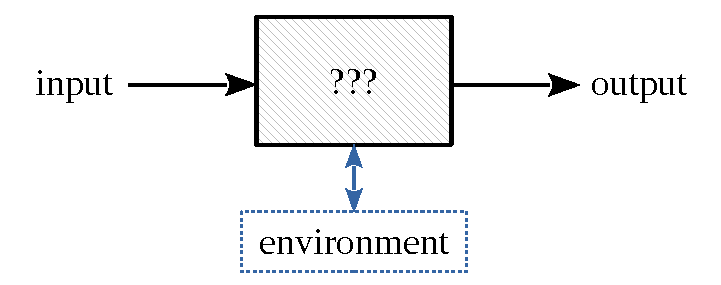
\includegraphics[width=0.9\linewidth]{images/blackbox} 
%    \caption{Black-box approach}
%    %\label{fig:sub1}
%  \end{subfigure}%
%  \begin{subfigure}{.5\textwidth}
%    \centering
%    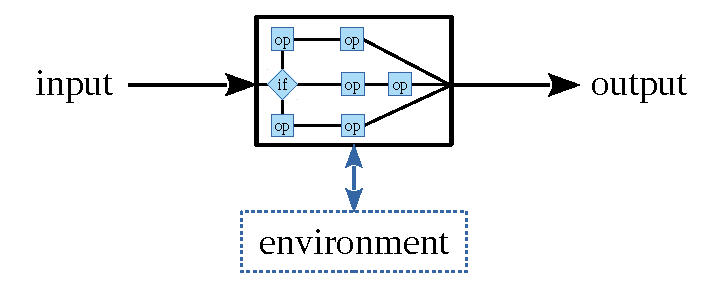
\includegraphics[width=0.9\linewidth]{images/whitebox} 
%    \caption{White-box approach}
%    %\label{fig:sub2}
%  \end{subfigure}
%  %\label{fig:example-symbolic-execution}
%  \vspace{-3mm}
%\end{figure}
%
%\paragraph{Taken from old Overview}
%
%Symbolic execution has been originally introduced in~\cite{K-CACM76} and~\cite{H-TSE77}. A good introduction to symbolic execution is presented in~\cite{KLEE-OSDI08}.\mynote{Extend this paragraph}
%%(while~\cite{EXE-CCS06} is a previous effort of the same authors).
%\cite{SAGE-NDSS08} is one successful story of symbolic execution. \cite{SAB-SP10} presents a neat formalization of symbolic execution and of taint analysis as well.
%
